\chapter{State of the Art}

\section*{\ac{CI/CD}}
In this chapter, the discussion will focus on the tools and technologies employed in this pipeline. 
Furthermore, other pipeline projects or Capture The Flag (CTF) challenges related to DevOps security will be introduced. 
Before diving into the tools utilized in this pipeline, 
the concept of Continuous Integration (\ac{CI}) and Continuous Deployment (\ac{CD}) will be introduced.

While \ac{CI} and \ac{CD} are distinct acronyms, they are often combined into one term because they are closely related and commonly occur together.
Continuous Integration (\ac{CI}) involves the continuous integration of code, where a set of practices, often automated, 
are implemented to integrate code changes. The term "continuous" in \ac{CI} refers to the ongoing nature of these practices 
rather than the code integration never stopping. \ac{CI} facilitates quicker feedback, 
enabling developers to observe their code in action promptly, making it easier to identify and rectify bugs and errors. 
The adoption of \ac{CI} doesn't necessarily mandate the use of sophisticated tools or pipelines; 
it simply promotes project agility and responsiveness to changes.\\
Continuous Deployment (\ac{CD}) is closely tied to \ac{CI}, as most software, when created, is ultimately exposed 
to users in some form, necessitating deployment. Thus, \ac{CD} complements \ac{CI}, ensuring that software changes 
are efficiently deployed and made available to users.\cite{duvall2007continuous}

The adoption of Continuous Integration and Continuous Deployment (\ac{CI/CD}) 
typically involves the implementation of a pipeline. A pipeline comprises a series of automated 
processes executed in a predefined sequence. It serves to automate tasks such as building, testing, and deploying software.\\
Constructing a pipeline entails utilizing a set of tools to establish an integrated infrastructure.
A pipeline can be as simple as a single script or as complex as a series of scripts orchestrated by a pipeline platform.\\
The tools discussed in this section are specifically those employed in the pipeline for this project. 
Notably, Ngrok, as discussed in Section \ref{sec:ngrok}, is the only tool not utilized in the final pipeline. 
However, its inclusion in this section is warranted as it played a role in addressing 
challenges encountered during the development of the remote pipeline (Section \ref{sec:pipeline_remote}) which not either in use.

\section{Tools}
\label{sec:tools}
\subsection{Docker}
\label{sec:docker}
Docker plays a pivotal role in this project, serving as an integral tool. 
It offers a clean and efficient means of running instances that essentially 
need to be isolated once they have completed their execution. 
This allows for the encapsulation of the machines or infrastructure used for the \ac{CTF} within Docker images, 
which can then be shared with other systems. When these images are executed on those systems, the expectation is to achieve consistent outcomes.

\subsubsection{What is Docker?}
Docker\cite{docker-docs} is an open platform used for developing, shipping, and running applications. 
It utilizes containers, which are isolated environments for running specific applications. 
Containers are lightweight and encapsulate everything needed for an application to run, 
eliminating the need for the host machine to have specific dependencies installed

\begin{figure}[h]
    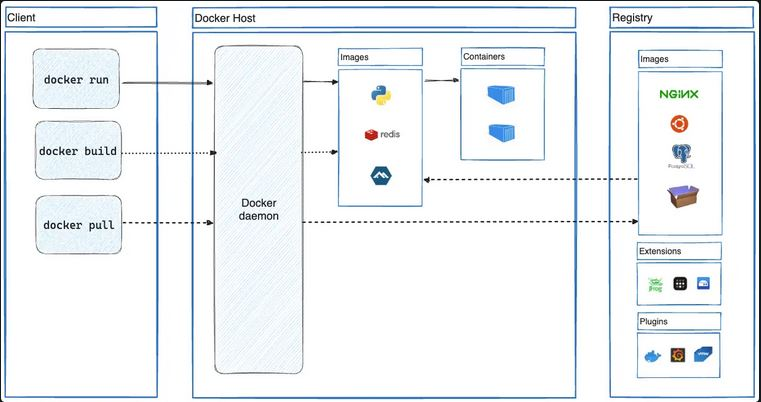
\includegraphics[scale=.7]{images/Docker-architecture.jpg}
    \caption{Docker architecture\cite{docker-docs}}
    \label{fig:docker_architecture}
\end{figure}

The architecture of docker is client-server. 
As seen in figure \ref{fig:docker_architecture} Docker consist of mostly 3 parts; client, daemon (host) and the registry.
The client is the \ac{CLI} which is used as an intermediary to communicate with the daemon. 
The daemon handles everything related to the containers, like building, running, and distributing them.
When images are not stored locally on a users machine or server, they are fetched from the registry.
The registry is a place where images are stored and can be fetched from. There is a many 
authorized registries, but the most common one is Docker Hub.\cite{dockerhub}\\
\paragraph{\textbf{What is a container?}}
A container\cite{docker-concepts} is an isolated process. 
That means that it's a process that runs on a host machine, but it's isolated from the host machine.
Containers can also be described as a lightweight \ac{VM}. Containers are also isolated from each other, but they share the same kernel.
Therefore containers act like components in a bigger project, meaning if a user wants to run a web-application, he or she might need a frontend, database, \ac{API}, etc.
All these things can be isolated from each other, but still have the ability to communicate with each other.
\paragraph{\textbf{What is an image?}}
A container is only as powerful as it's configuration, and for configuring a containers,
Docker uses images\cite{docker-concepts}.\\
Images are the configuration of the container.
They are used to create containers. Images are read-only, meaning that they can not be changed once build.
To change an image, one would to rebuild it from scratch.
For Docker to work, the parts has to work together in harmony. The client sends a request to the daemon, which then executes the request.
If the image isn't stored locally it fetches it or builds it. Once an image is locally present and complete the daemon  
will create a container from the image.
When using the Docker CLI things can quickly become complicated, but with the help of \javaf{docker-compose}, things can be simplified.
\subsubsection{\javaf{docker-compose}}
Docker compose is a tool for running multi-container applications. With the help of \ac{YAML}\cite{YAML}
and a configuration file name \javaf{docker-compose.yml}, it is possible to define services to run.
The docker compose\cite{docker-compose} application model consist of the main 3:
\begin{itemize}
    \item \javaf{Services} is a definition of a containerized application or components of an application. For the Docker compose file,
    this is where the definition of the services that going to be spawn that make the \javaf{docker-compose} file a multiple container application.
    \item \javaf{Networks} is a definition of a virtual network that containers can connect to, in order to communicate with each other.
    If no network is specified, the containers will be connected to the default network. In Docker compose it is possible for 
    containers via Docker internal \ac{DNS} to communicate with each other. 
    This means that even though that IP's might change, the containers can find and communicate with another container through it \ac{DNS} record.
    \item \javaf{Volumes} are a way to persist data generated by containers or share data between containers and the host system. 
\end{itemize}
When combining these three elements, it is possible create a multi-container application. The \javaf{docker-compose} file is a 
\ac{YAML} file that defines the services, networks, and volumes that is going to spawned. Once a developer
has defined everything needed in the \javaf{docker-compose} file, the multi-container application 
can be spawned with a single command, \javaf{docker-compose up}. As there can be many ways to define a \javaf{docker-compose} file, 
we'll wait until section \ref{sec:technical_implementation} to see the \javaf{docker-compose} file that is used in this project.
\newpage

\begin{itemize}
    \item First: Gitea is an open source project and is there subjective to changes at any time. For this project,
    I need to ensure that the end result is the same as when I started the project. 
    To circumvent this, the base image of Gitea is chosen to be version 1.16.5. Now why this version? 
    Based some testing it seems that most of the API admin options are unavailable in version later than 1.19.0. Version between 1.16.5 and 1.19.0
    have changes which impacts the use of admin API options.
    Using the version 1.16.5 Docker image esnure that even though long time developing this project, the base image stay the same and 
    the end result will be same as when i started the project, and when the user pulls the image.
    \item Second: The configuration of Gitea needs to be static. When Gitea is installed, it will prompt the installer of Gitea 
    to specify what that person wants. This information will be stored in a special file called app.ini. This file is 
    used by Gitea to configure itself\ref{fig:gitea_app_ini_remote}. The rest of the app.ini file for this project
    can be found the source code of the project under Gitea/app.ini.
    \item Third: Users needs to be created at initialization, so that when the user start the image via docker-compose. 
    The database is already populated with users, and the user can start using the service right away.
    This is done with python3\cite{python} script which 
    post users to the database via a \ac{RESTAPI}, with admin credentials.
\end{itemize}

\subsection{Drone problems}
\label{sec:discussion-drone}

\subsubsection{Deployment on drone}
The newest version of the Drone server uses Oauth2 to authenticate user account to the server.
This means that another entity, such as gitea authenticates user to the Drone server. This is done by
setting up a Oauth2 application in gitea, and then using the client id and client secret to authenticate
the user to the Drone server. On the Drone official website, it states that it is not recommend to deploy 
Drone with docker-compose, because of the potential network issues that might arise.
\paragraph{Problem 1, integration with gitea over OAuth2}
Other than starting out figuring out how to run Drone, I had to figure out how to integrate it with gitea.
Now later version of Drone, had its own database of users and therefore didn't have to rely on gitea for authentication.
Now this means that before being able to run Drone runners to execute pipeline, the user that wish to use Drone,
needs to authenticate with the gitea server, and post a access token to the gitea server. Essentially the user needs a token 
when is used to authenticate with the gitea server.
Now the authentication process is not a problem, the Drone CI/CD documentation is very specific about how to do it and if done 
correctly it'll work fine.
Now the big problem is posting the token to the gitea server. The gitea server will not accept the token, being posted over http connection,
and it refusing the connection. 
Since Drone need to make it's access token available to the gitea server, it needs to be able to post it to the gitea server.
The problem can be solved by using a proxy or a https connection on the gitea server, but that is not a viable solution.

\paragraph{Problem 2, Advertised problem by Drone}
Now the is linked to the first problem and is about the network aspect of Drone.
The authentication of the user is done in the browser. When that is done Drone obviously needs to be able to communicate with the gitea server.
Now the problem, and im not sure how docker compose works in this part, but what I've deciphered from the internet is that 
Drone might not be able to find the gitea server, and post the token to it.

\paragraph{Problem 3, Drone runner}
When the Drone server is operational, it acts as the intermediary connecting the Git server 
and the runners responsible for executing the pipeline. 
To ensure a smooth pipeline execution, it is imperative that the pipeline configuration 
for the Drone server is exceptionally detailed. This configuration should explicitly define 
crucial details such as the software used to manage the Drone server, particularly Docker if the Drone runners 
are tasked with running the pipeline within Docker containers.

Furthermore, the fact that this specification must be written in YAML introduces a 
level of dependency on YAML syntax and indentation. It's important to note that the 
specific syntax and indentation requirements can vary from one software platform to another when defining the structure of the pipeline. 
Therefore, careful attention to these details is vital to ensure accurate and effective pipeline execution.

\subsection{Ngrok}
\label{sec:ngrok}
Ngrok was used is this product to expose the local Gitea server to the internet. This was done to allow remote access to the server.
Ngrok is a multiplatform tunnelling, reverse proxy software that establishes secure tunnels from a public endpoint to a local running network service.
Ngrok acts as a unified ingress platform combining all the components to deliver traffic from local service to the internet. 
Ngrok consolidates together the reverse proxy, load balancer, \ac{API} gateway, firewall, delivery network, DDoS protection and more.\cite{ngrok}

\subsubsection{How does Ngrok work?}
Ngrok is a reverse proxy but there is a little more to it than just that. Ngrok 
works on a global network called the \javaf{Ngrok edge}. At the edge, traffic is accepted from client from the internet 
and then forwarded to the local service.
Unlike traditional proxies Ngrok does not transmit traffic to an upstream application by forwarding IP address. Instead, 
Ngrok is a small piece of software that you run along side a local application. This software will connect to 
the Ngrok edge and will keep the connection open. When a client connects to the Ngrok edge, the edge will forward the
traffic to the local application.
There are four ways of running the client\cite{ngrok-works}.

\begin{itemize}
    \item As a service: Run as a small side process called the Ngrok agent as a
    background \ac{OS} service.
    \item As an interactive \ac{CLI}: Run as the Ngrok agent
    interactively from the command line while developing and testing.
    \item As an \ac{SDK}
    embedded in your app: Included as a small Agent \ac{SDK} library directly into an
    application software that returns a socket-like object. 
    \item As a Kubernetes
    Controller: Run the Ingress Controller in a Kubernetes environment.
\end{itemize}

In this project, the Ngrok agent was run as a service. This was done to ensure that the connection to the Ngrok edge was at all times.

\subsection{Nginx proxy}
\label{sec:nginx}
Nginx is a reverse proxy, serving as the intermediary between the client and the internal network where the application runs. 
It manages the DNS records requested and directs the traffic to the corresponding IP address. 
Consequently, the client is unaware of the application's IP address, knowing only the gateway. This gateway is a docker network gateway.
The client sends a request to the application via HTTPS. 
The proxy forwards this request to the application, which then sends the response back to the proxy. 
This setup adds an extra layer of abstraction, helping to protect the internal network from the outside world.
It also gives the possible to add more infrastructure to the application, such as load balancing, caching, certificates handling and more.\\

\paragraph{Passing a request to a proxied server}
Whenever nginx receives a request, it tries to find the server that the request should be forwarded to.
The server is specified in the \javaf{proxy_pass} directive. The \javaf{proxy_pass} directive is used to specify the server that the request should be forwarded to.\\
Simply what the \javaf{proxy_pass} specification does, is the declaration of the server that the request should be forwarded to.
That can either be a \ac{DNS} record or an \ac{IP} address.\cite{nginx-proxy-3}

\paragraph{Configuring buffers}By default NGINX buffers responses from upstream servers.
A response is stored in the internal buffers and is not sent to
the client until the whole response is received. Buffering helps to optimize performance with slow clients, 
which can waste upstream servers time if the response is passed from NGINX to the client synchronously. 
However, when buffering is enabled, NGINX allows the upstream servers to 
process responses quickly, while NGINX stores the responses for as much time as the clients need to download them.\cite{nginx-proxy-3}
The specification of these buffers are noted in the configuration as seen in figure \ref{fig:buffer-config}.
\begin{figure}
    \begin{center}
        \javaf{proxy_buffers $size$ $number$;} \\
        \javaf{proxy_buffer_size $size$;}.
    \end{center}
    \caption{Configuring buffers}
    \label{fig:buffer-config}
\end{figure}
The specific configuration for the this project will be covered in section \ref{sec:pipeline-local-nginx}.

\subsubsection{Docker gateway}
\label{sec:gateway}
For the NGINX reverse proxy to function, it needs a gateway to attach itself to. Here the Docker network is used as the gateway.
The Docker network is a virtual network that is created by Docker. The network is used to connect containers together.
The network is created by the Docker daemon when the first container is created. The network is created with the name \javaf{bridge}.
The bridge network is the default network that is created by Docker.
The bridge network is a \ac{NAT} network that is used to connect the containers to the host.

\subsection{Registry}
\label{sec:registry}
The Drone pipeline when using Docker runner needs a registry to pull and push images to.
The default registry that is used is the Docker hub. Because the future work of the project includes
having the project running on haaukins (Section \ref{sec:haaukins}) which does not have internet when running.
Here in comes a local registry. A local registry will resides as a mirror of Docker Hub, when 
other container which has docker installed is made aware of the local registry, it will pull images from the local registry.
If no internet connection is available, the Drone runners will not be able to pull images from the docker hub. 
How this is solved is either by providing all container with the address of the mirror registry of Docker hub or 
using specific \ac{URL} for the desired images in the pipeline.\\
\paragraph{What is a registry?}
A registry is a storage and content delivery system, holding named Docker images, available in different tagged versions.
The registry is a stateless, highly scalable server side application that stores and let you distribute Docker images.
The registry is open-source, under the Apache 2.0 license. Some of the features of the registry are:

\begin{itemize}
    \item The ability to store images in a central location.
    \item The ability to control access to the images.
    \item The ability to integrate image storage and distribution into the \ac{CI/CD} pipeline.
\end{itemize}

\newpage

\subsection{Certificate}
\label{sec:certificate}
Certificates are used for all websites that run \ac{HTTPS}. 
The certificate is used  to let visitors know that the website is secure.
The certificate has associated cryptographic keys that are used to encrypt the data being transferred between the client and the server.
Futhermore, the certificate might be signed by a \ac{CA} which is a trusted third party.
When a client connects to a website that uses \ac{HTTPS}, the client will check the certificate
to see if it is signed by a trusted \ac{CA}. If the certificate is signed by a trusted \ac{CA}, the client
will trust the website. If the certificate is not signed by a trusted \ac{CA}, the client will get a warning
that the website is secured by a self signed certificate.\\
There are various methods to create a certificate, and no single approach is definitive. 
For this project, a self-signed certificate was created to enable HTTPS connections between all services \cite{self-signed-cert}.


\paragraph{Self signed certificate}
When creating a self signed certificate, access to the server or the proxy that is going to handle the certificate is necessary.
The certificate is created using the openssl command first one will have to create a private key:
\begin{figure}[h]
    \begin{center}
        \javaf{openssl genrsa -out eds.key 2048}
    \end{center}
    \caption{Creating a private key}
    \label{fig:private-key}
\end{figure}
The private key created in figure \ref{fig:private-key} is a RSA key that is 2048 bits long. 
Normally, the private key would be encrypted with a password, but for this project, 
the private key will not be encrypted to avoid the need to enter a password during deployment.
Next, a Certificate Signing Request (CSR) will be created. 
A CSR is an encoded file containing information about the organization requesting the certificate \cite{csr}. 
The CSR is sent to a Certificate Authority (CA) for signing. In this case, the certificate will be self-signed.
\begin{figure}[h]
    \begin{center}
        \javaf{openssl req -key eds.key -new -out eds.csr}
    \end{center}
    \caption{Creating a CSR}
    \label{fig:csr-creation}
\end{figure}
When creating a \ac{CSR}, openssl ask for information to be filled. This information is about the creator of the CSR.
The information that is asked for is:
\begin{itemize}
    \item Country Name (2 letter code) [AU]: 
    \item State or Province Name (full name): 
    \item Locality Name (eg, city): 
    \item Organization Name (eg, company): 
    \item Organizational Unit Name (eg, section): 
    \item Common Name (e.g. server FQDN or YOUR name): 
    \item Email Address:
    \item A challenge password:
    \item An optional company name:
\end{itemize}
\ac{CN} is the domain name which the certificate is going to be used for.
After the private key and \ac{CSR} is created, we can create the certificate. We created the certificate using \javaf{x509} format.\\
\javaf{x509}\cite{x509} is standardized format for public key certificates. What \javaf{x509} certificate provides is the ability
to both create a self signed certificate, but also allow our application to be accessed through \ac{HTTPS}.\\
\begin{figure}[h]
    \begin{center}
    \javaf{openssl x509 \ }\\
    \javaf{-signkey eds.key \ }\\
    \javaf{-in eds.csr \ } \\
    \javaf{-req -days 365 -out eds.crt}
\end{center}
    \caption{Creating a certificate}
    \label{fig:cert-creation}
\end{figure}
The certificate, created by the command seen in figure \ref{fig:cert-creation}, is designed for a single page. 
To support multiple websites under various domains within the same subdomain, 
a certificate endorsed by a Certificate Authority (CA) is required.\\
Having the created certificate signed by 
a CA allows the association of the desired subdomain, enabling an unlimited number of subdomains. 
The initial step involves generating a new private key and self-signing 
an CA certificate, which will be used to endorse the previously created certificate.
Now that a CA certificate called edsCA is created by the command seen in figure \ref{fig:ca-cert}.
edsCA can be used to sign the certificate that was created in figure \ref{fig:cert-creation}.\\
\begin{figure}[h]
    \begin{center}
        \javaf{openssl req -x509 -sha256 -days 1825 \ } \\
        \javaf{-newkey rsa:2048 -keyout edsCA.key -out edsCA.crt}
    \end{center}
    \caption{Creating a CA certificate}
    \label{fig:ca-cert}
\end{figure}
A configuration file, named \javaf{eds.ext}, will be used to add additional information to the certificate. 
The \javaf{eds.ext} file contains the following information:
\begin{figure}[h]
    \begin{center}
        \javaf{basicConstraints=CA:FALSE} \\
        \javaf{extendedKeyUsage=serverAuth} \\
        \javaf{subjectAltName = *.devops.eds}
    \end{center}
    \caption{Data for configuration file for the CA certificate}
    \label{fig:ca-cert-ext}
\end{figure}
\javaf{extendedKeyUsage} is serverAuth because we're going to use ssl/TLS authentication a server.
\javaf{basicConstraints} is set to false because the certificate is not a valid  CA certificate.\\
\javaf{subjectAltName} is the domain name that the certificate is going to be used for.\\\cite{openssl-ext}
\begin{figure}[h]
    \begin{center}
        \javaf{openssl x509 -req -CA edsCA.crt \ } \\
        \javaf{-CAkey edsCA.key -in eds.csr \ } \\
        \javaf{-out eds.crt -days 365 \ } \\
        \javaf{-CAcreateserial -extfile eds.ext}
    \end{center}
    \caption{Signing eds.crt with edsCA.crt}
    \label{fig:sign-cert}
\end{figure}

The command from figure \ref{fig:sign-cert} takes a CSR (eds.csr), signs it using the CA certificate 
(edsCA.crt) and its private key (edsCA.key), and generates a signed certificate 
(eds.crt) valid for 365 days, including any specified extensions from the eds.ext file.\\
This certificate has been signed with the CA certificate, 
meaning that if it is placed in \javaf{/etc/ssl/certs/ca-certificates.crt} on Linux, the system will trust the certificate.

\section{CI/CD CTF Pipeline}
\label{sec:ci-cd-ctf-pipeline}
As this project focuses on the development of a pipeline for the creation and deployment of \ac{CTF} challenges, 
it is essential to understand the available pipeline platforms, that are already out there. 
Even though there may not be an existing pipeline exactly 
like the one being developed, it is still important to understand what other tools can and cannot do. 
In this section, I will briefly some of the pipelines that I consider noteworthy. 
These pipelines have some merits in terms of what I believe a pipeline should be able to do and what it should not do.


\paragraph{CICD-Goat}
\label{par:cicd-goat}
The CICD-Goat\cite{cicd-goat} is one of the other \ac{CTF} pipelines that is out there.
The pipeline is created based on the OWASP Top 10 CI/CD security risk\cite{owasp-cicd-top-10} list.
The pipeline is aimed toward developers, security professionals, and others who are interested in understanding the \ac{CI/CD} pipeline.
The pipeline is constructed with technology of Gitea, Jenkins, Gitlab and Gitlab runners.
The pipeline infrastructure is build inside Docker containers and used localhost to export the website.
It used a local instance of CTFd to host the challenges and report the flag.

The CICD-goat project has a lot of merit in the sense that they focus on real proven scenarios that 
is happening to pipelines in productions settings, anyhow the project uses an old technology in Jenkins. Jenkins 
is a great tool, but in the sense of a modern pipeline and pipeline structure, Jenkins is outdated.

\paragraph{Poursoft}
\label{par:poursoft}
Poursoft is the recent create pipeline for the national \ac{DDC}. It was created by Oliver Nordestgaard
and was used in the national \ac{DDC} 2024. The pipeline utilize many of the same tools as the pipeline for this project.
The pipeline is not open-source and can't be referenced in this project. Although through my work on \ac{DDC} 2024,
I had access to the repository and could see how the pipeline was constructed. The pipeline was constructed with the following tools:
\begin{itemize}
    \item \javaf{Gitea} as the git repository.
    \item \javaf{DroneCI} for the pipeline
    \item \javaf{Ngnix} for a websever and reverse proxy
    \item \javaf{Haaukins} for the deployment of the challenges
\end{itemize}

\paragraph{Tryhackme, Hackthebox, and other commercial projects}
\label{par:tryhackme-hackthebox}
TryHackMe and Hack The Box are both commercial platforms and are not open-source. They require a subscription fee for access.
On TryHackMe\cite{tryhackme}, it is possible to view available challenges without logging into the website. 
TryHackMe offers numerous challenges relevant to pipelines. While not directly focused on pipelines, 
these challenges involve tools commonly used in pipelines, such as Docker, Kubernetes, GitLab, DevSecOps practices, and more.\\
Hack The Box\cite{hackthebox} primarily focuses on the exploitation of machines. After exploring their website, it appears they have a few 
DevOps-related challenges. However, 
the specific focus of these challenges is not clearly indicated, making it difficult to assess their relevance to DevOps Capture The Flag (CTF) events.



\newpage
